\chapter{Simulation}
\minitoc
\label{Cap:Simulation}

\section{Introduction}
\label{Cap:Simulation:Introduction}
The simulation of the MINER$\nu$A detector has multiple functions, such as background estimation, efficiency detector studies, simulation of reconstruction and the comparison of different  model with data. In this Chapter the different steps of the MINER$\nu$A experiment simulation are explained, including the beam simulation and a brief description of the models used by the simulators.

The simulation starts with the beam simulation, followed by the neutrino interaction simulation inside of the MINER$\nu$A detector geometry. It proceeds with the simulation of the propagation of the resultant particles in the interaction with the detector, here the deposited energy, the particles track and secondary particles are simulated. The last part of the simulation consist in a decalibration of the results from the previews stage in the way to simulate the same conditions of the real detector. At the end, it returns the simulated data in the same format that the raw data. In the following sections, the simulation steps are explained.

\section{Beam simulation}
\label{Cap:Simulation:BeamSimulation}

The neutrino flux simulation is performed in G4NuMI, based in GEANT 4 \cite{GEANT4}. In this stage the production of hadrons, the focusing and the secondary interactions of the hadrons with the different components of NuMI are simulated. It starts giving as input the proton beam from Main Injector and finishes with the neutrino beam. The output from the simulation is dk2nu format \cite{dk2nu}. The output includes information about the kinematics of the neutrino, the ancestors of the neutrino, paths through magnetic field and reinteractions of the mesons with the components of NuMI. This information is used by GENIE\cite{Genie} as input in the next stage of the simulation to simulate the neutrino interaction simulation in the detector.
 
After to give the as input the proton beam from Main Injector, which corresponds to a 120 GeV kinetic energy with a Gaussian transverse profile distribution with $\sigma$ = 1.1 mm, continuing with the hadron production simulation. For the hadron production, GEANT 4 use the hadronic model FTFP\_BERT that is a combination of the FRITIOF \cite{PhysRevD.90.032001} and Bertini \cite{BERTINI1971670} \cite{GUTHRIE196829}cascade models. However, the reinteractions of the mesons with other components of NuMI are not well simulated, because these interactions are modeled by non-perturbative QFT. The \textbf{Figure} \ref{fig:Simulation:Beam:HadIntperNu} shows the simulated number of hadronic interactions per neutrino as function of the neutrino energy, from the figure the predominance of the $pC\rightarrow\pi X$ for the hadrons that produce the ME beam can be observed. 

\begin{figure}[!htb]
    \centering
    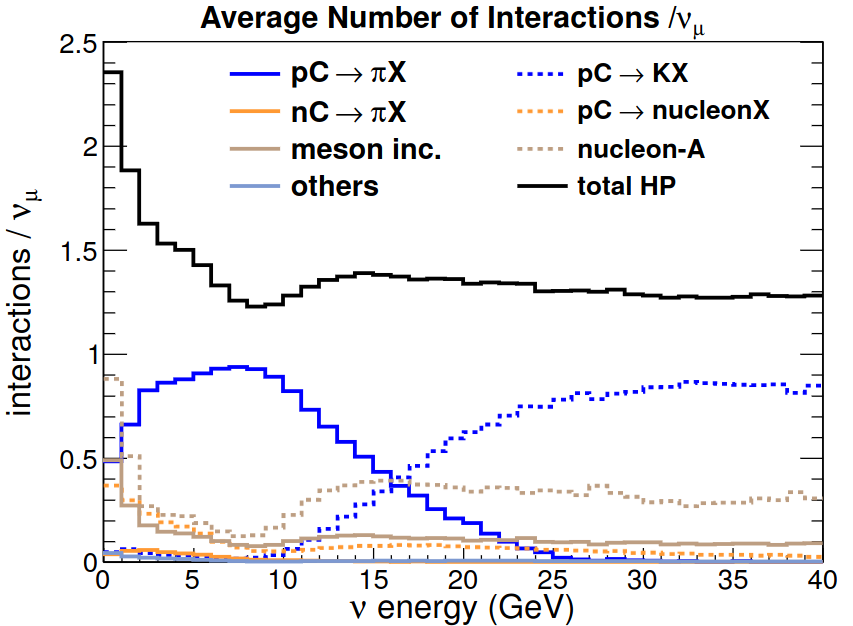
\includegraphics[scale=0.3]{Figures/Chapter3/HadronicInteractions.png}
    \caption{In this plot the simulated number of hadrons interactions per neutrino as function of the produced neutrino energy for the ME era are shown. Figure from \cite{LeoThesis}}
    \label{fig:Simulation:Beam:HadIntperNu}
\end{figure}

The current solution to constraint the models is to use the data obtained from NA49\cite{NA49}. In this studies \cite{NA49} the cross section results for the charge pion production are shown, the interest of in the production of the charge pions is because it is the dominant source of neutrinos at the neutrino beam. The pion yield, $f_{Data}$, from NA49 inelastic interactions is obtained by

\begin{equation}
    f_{Data}=E_\pi\frac{1}{\sigma_{inel}}\frac{d^3\sigma}{dp^3},
\end{equation}

where $E_\pi$ is the pion energy, $\sigma_{inel}$ is the total inelastic cross section, $p$ is the proton momentum. For the MC we have the equivalent relation. In the way to obtain the weight for the meson that produce the neutrino is 

\begin{equation}
    weight(x_F,p_T,p) = \frac{f_{Data}(x_F,p_T,p_0=158 GeV)}{f_{MC}(x_F,p_T,p_0=158 GeV)}s(x_F,p_T,p),
\end{equation}

where $x_F$ is the Feynman variable; $s$ is a factor scale the 158 GeV to 120 GeV that corresponds to the Main Injector proton beam, it is calculated by FLUKA\cite{Fluka}; $p_T$ is the transverse momentum. 
\textcolor{red}{Hablar mas sobre la simulacion del beam, hablar sobre las diferentes fuentes de errror.  Puede ser aqui o en una pendice como lo hace Ben}
 
\begin{figure}
    \centering
    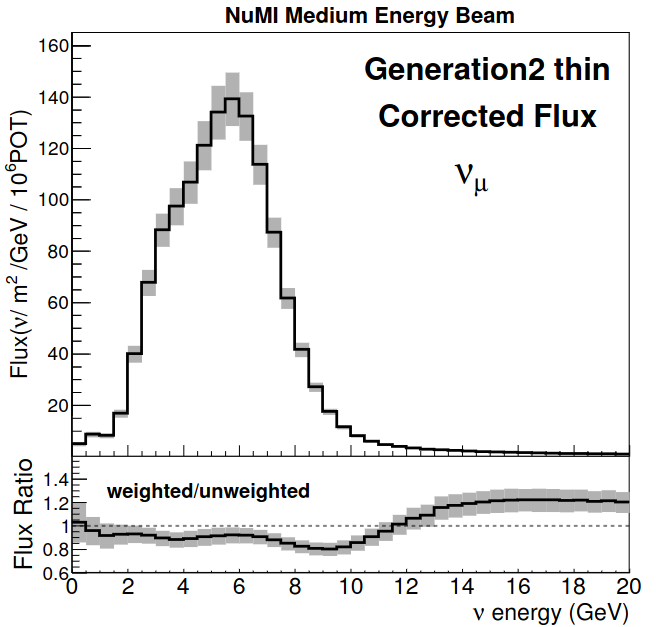
\includegraphics[scale=0.3]{Figures/Chapter3/FluxDistribution.png}
    \caption{Simulated neutrino flux distribution as function of the neutrino energy for the ME era. Figure from \cite{LeoThesis}}
    \label{fig:Simulation:Beam:FluxDistribution}
\end{figure}

\section{Interaction Simulation}
\label{Cap:Simulation:InteractionSimulation}

After to simulate the neutrino beam, the next step is simulate how those neutrinos interacts with the MINER$\nu$A detector, this part of the simulation is made using GENIE\cite{Genie}. GENIE brings information about the neutrino interaction, vertex kinematics, particle identities, the initial particles state, the ancestors of the particles, interactions inside of the nucleus and the final state particles kinematics. The results reported for this thesis include the MINER$\nu$A detector  simulation using the GENIE version 2.12.6. GENIE is described with more detail in the \textbf{Subsection} \ref{Cap:Simulation:GENIE}.

\subsection{GENIE}
\label{Cap:Simulation:GENIE}
GENIE is a neutrino event simulator based on ROOT in C++ language. GENIE is capable to simulate neutrino interactions for a large range of neutrino energy spectrum. This being very useful for a large number of experiments. The physics models used by GENIE can be categorized into nuclear physics models, cross section models and hadronization models.






\section{Detector Simulation}
\label{Cap:Simulation:DetectorSimulation}

\subsection{GEAN 4}
\label{Cap:Simulation:GEANT4}

\section{MC reconstruction}
\label{Cap:Simulation:MCReconstruction}




